% KTrack documentation for the Kassiopeia Guide
\setcounter{secnumdepth}{4}
\section{Particle Tracking: KTrack}\label{sec:KTrack}

KTrack is a program package to compute particle trajectories. The program is valid for any type of particle.

KTrack was developed for simulating the motion of particles in the KATRIN experiment; therefore, the implemented equations of motion describe particle motion in electro magnetic fields. The framework of KTrack, however, allows for implementing an arbitrary equation of motion. 

For solving the equation of motion the user can choose, at present, between six ODE solving methods: \textit{8th order Runge-Kutta}, four different \textit{Emmbedded Runge-Kutta Methods} (\textit{4th/5th order Runge-Kutta}, \textit{5th/6th order Runge-Kutta}, \textit{6th/8th order} and \textit{8th/7th order Runge-Kutta}) and \textit{Predictor-Corrector}. The latter five provide an intrinsic numerical time step control. In addition to these controls, a number of criteria for determining the time step are offered by KTrack. The user can choose to control the step size by means of energy conservation, a global limit on the step size, a fraction of the cyclotron period, limits on the energy loss due to synchrotron radiation, and limits on scattering probability. Any combination of controls can be chosen.

KTrack offers two main computation modes. Firstly, there is an exact trajectory calculation based on solving the Lorentz equation. Secondly, there is a mode which is based on computing the guiding center motion. It makes use of the adiabaticity of the motion, i.e. the conservation of the first order orbital magnetic moment. In this mode magnetron drift motion and gyration are added seperately. A third mode, in which the drift motion is embedded in the equation of motion, will be added in the near future. 
 
The program package also includes elastic and inelastic scattering on hydrogen. Any other scattering module can be added easily. Synchrotron radiation is optionally taken into account in the calculation.

The mathemathical description of the physical processes is taken from Ferenc Gl\"uck's c-language routines.

People involved in developing KTrack:
John Barrett, Daniel Furse, Ferenc Gl\"uck, Wolfgang K\"afer, Benjamin Leiber, Susanne Mertens, Nancy Wandkowsky

\subsection{KTrack's general structure}

In this most recent version, KTrack has been reorganized into a general modular framework.  The basic unit of this framework is called a \textit{Process}, which generally represents any action that changes the state of a particle.  For example, propagating a particle according to an equation of motion using a differential equation solver is a kind of \textit{Process} called, more specifically, \textit{Propagation}, which changes the particle's position and momentum.  The effect of synchrotron radiation loss during a step is likewise encapsulated in a \textit{Process}, called \textit{Synchrotron}.  Its action is to reduce the transverse momentum of a particle.

In addition to the examples above, which are self-contained \textit{Processes} representing specific physics, the \textit{Processes} in KTrack can be combined into composite tree structures.  To give an example, the \textit{Adiabatic Stepping Method} itself is treated as a \textit{Process} in KTrack, and it sits at the base of a tree whose branches represent sub-\textit{Processes}.  In the case of the \textit{Adiabatic Stepping Method}, these branches are a \textit{Propagation Process}, possibly a \textit{Synchrotron Process}, possibly a \textit{Drift Process}, a \textit{Gyration Process}, and finally, possibly a \textit{Scattering Process}.  This tree-like structure is realized in C++ according to the \textit{Composite} pattern, described in \ref{compsite}.

As mentioned above, there are various criteria to control the step size available in KTrack.  The basic behavior of these controls is captured in a class called \textit{StepSize}, and each step size naturally belongs to a particular \textit{Process}.  For instance, the energy conservation step control naturally belongs to \textit{Propagation}, and the synchrotron radiation step size control naturally belongs to \textit{Synchrotron}.  Each of these controls is able to suggest a time step, which is that control's best guess at the maximum time step it itself can tolerate.  Each control is also able to examine whether the action of its parent process has exceeded the control's tolerance, at which point it can veto the step and make an improved suggestion for the step size.

The methods of all classes can be classified as following types:
\begin{itemize}
    \item action: 
        \begin{itemize}
            \item initialize processes
            \item changing the state of the particle
            \item reset processes
            \item compute time step
        \end{itemize}
    \item composition       
        \begin{itemize}
            \item add processes/step size controls
            \item remove processes/step size controls
            \item get processes/step size controls
        \end{itemize}
    \item identification
        \begin{itemize}
            \item get name of class
            \item get type of class
            \item get name of parent class
        \end{itemize}
    \item configuration
        \begin{itemize}
            \item set parameters
            \item set field calculation method
            \item set cross section calculation method
            \item etc.
        \end{itemize}
    \item delegation:  methods called by child process to get information about the parent process 
        \begin{itemize}
            \item e.g. returns pointer to the ODE that is used
            \item e.g. returns pointer to intermediate particle
            \item etc.
        \end{itemize}
\end{itemize}

Further technical details and discussion of how the tree-like structures of \textit{Processes} are composed; how \textit{StepSizes} are attached and configured, and how initialization generally occurs within such structures can be found in the following chapters.

\subsection{KTrack Step Computer}
\label{ktrackstep}  

A \textit{KTrack Step Computer} is itself of the type \textit{Process}; the class \textit{KTrackStepComputer} inherits from \textit{Process}. A full step is composed of a number of sub processes. To perform a step \textit{KTrack Step Computer} has the following public method:
    \begin{itemize}
        \item Execute()
    \end{itemize}
    To organize sub processes \textit{KTrack Step Computer} has the following public methods:
    \begin{itemize}
        \item AddProcess(*process)
        \item RemoveProcess(std::string processname)
        \item GetProcess(std::string processname)
    \end{itemize}
    KTrack has two tracking methods, so far, the exact and adiabatic method, (these are described in more detail below, see \ref{exactadiabatic}). The corresponding classes \textit{ExactStep} and \textit{AdiabaticStep} inherit from the base class \textit{KTrackStepComputer}. As a private member, they have a vector of pointers to the processes that are activated by the user.
    
    When calling \textit{Execute()} on an exact or adiabatic step object following actions take place:
      \begin{itemize}
        \item Check whether the current step is the first step of a track:
        \begin{itemize}
            \item If yes: initialize intermediate particles (see \ref{intermediate particles}) and ODE
            \item If no: use the final state of the particle from the step before
        \end{itemize}
        \item Do while:
        \begin{itemize}
            \item compute the time step: ask the \textit{StepSizeOrganizer} to return the smallest suggestion of a time step from all activated step size controlers (see \ref{stepsizes}) 
            \item execute all activated processes: call \textit{Execute()} on all processes of the vector of processes in the right order. If the execution fails the step size control that failed reduces the time step and the program continues at the beginning of the while loop.
        \end{itemize} 
        \item Update intermediate and basic particle (see \ref{intermediateparticle})
      \end{itemize} 
        
    By calling \textit{AddProcess(*Process)} the process given in the argument is added to the vector of processes. This allows for switching on a process (e.g. scattering) in a certain region. It checks whether this process can be added, i.e. it checks if the process is applicable for the chosen stepping method - one could not add \textit{Drift} to the exact stepping method - and whether this process has already been added. It also takes care of the ordering of the processes, by putting the process in the right position of the vector of processes. To realize the ordering, the entires of the vector are couples of pointers to the \textit{processes} and a string, that describes with process is allowed to be at this position. 
    
    \textit{RemoveProcess(std::string processname)} removes a process from the vector. \textit{GetProcess(std::string processname)} returns a pointer to an object with the corresponding process name. With the help of this method, one can change the settings of the processes during run time.
    
    
    \subsubsection*{Exact and adiabatic stepping method}
    \label{exactadiabatic}   
    As mentioned, KTrack has two different stepping methods. One method, called \textit{Exact Stepping Method}, computes the exact trajectory, by solving the Lorentz equation. The other one, called \textit{Adiabatic Stepping Method}, computes the guiding center motion of the particle and adds the gyration in as a separate \textit{Process}. Here, the magnetron drift of the particle can optionally be swiched on. Both methods offer the possibilty to take synchrotron radiation and scattering processes into account. The adiabatic method has the potential to be much faster compared to the exact method, since it allows for much larger step sizes.
    
    Technically, there are only three differences between the adiabatic and exact stepping method:
    \begin{itemize}
         \item The ordered set of sub-processes is different: 
         \begin{itemize}
             \item In the case of the exact stepping method the only possible processes are: \textit{Propagation}, \textit{Synchrotron} and \textit{Scattering}. 
             \item For the adiabatic stepping method \textit{Propagation}, \textit{Drift}, \textit{Synchrotron}, \textit{Gyration}, and \textit{Scattering} are possible.
         \end{itemize} 
         \item Exact step and adiabatic step work with the so-called \textit{Exact Step Particle} and the \textit{Adiabatic Step Particle}, respectively. See chapter \ref{intermediateparticle}.
        \item Different ODEs are used in the process \textit{Propagation}:
        \begin{itemize}
            \item \textit{Exact Stepping Method} uses the Lorentz equation: 
                \begin{eqnarray}
                    \dot {\vec{x}} &=& \vec{v} \\
                    \dot {\vec{v}} &=& q \left(\vec{E} + \vec{v} \times \vec{B} \right) 
                \end{eqnarray} 
            \item \textit{Adiabatic Stepping Method} uses:
                \begin{eqnarray}
                    \dot {\vec{x}} &=& \hat{B} v_{\mathrm{long}} \\
                    \dot {v}_{\mathrm{long}} &=& -\frac{\mu}{\gamma} \left(\vec{\nabla} |\vec{B}| \right) \hat{B} + q \vec{E} \cdot \hat{B}
                \end{eqnarray} 
        \end{itemize}
        
    \end{itemize}  

\subsection{Processes}
\label{processes}
A step is composed of a number of \textit{Processes}:
\begin{itemize}
\label{listofprocesses}
    \item Propagation
    \item Synchroton radiation
    \item Elastic and inelastic scattering processes
    \item Magnetron drift motion (only needed for adiabatic stepping method)
    \item Gyration motion (only needed for adiabatic stepping method)
\end{itemize} 

The processes are structured in a common way. This is reflected by the fact that they all inheret from the common base class \textit{Process.h}. All processes share the method \textit{Execute()} which performes the required calculations and updates the affected particle properties.

In both the adiabatic and exact KTrack mode (see \ref{modes}) a step begins with the \textit{Propagation}. After the propagation, \textit{Synchroton} radiation is executed. In the case of the adiabatic method the \textit{Drift} (optionally) and \textit{Gyration} are executed afterwards. Finally \textit{Scattering} is executed. 

The set of \textit{Processes} can be divided into two man subsets. One is the \textit{Propagation}, performed by solving an equation of motion. The other \textit{Processes}, such as \textit{Synchrotron Radiation}, \textit{Scattering}, \textit{Magnetron Drift Motion} and \textit{Gyration Motion} are treated as corrections to the \textit{Propagation}.  They actually take place during the propagation, however, in the code they are added after the propagation has already been performed. To reflect reality best, these processes need information about the state of the particle at the beginning (initial particle) and at the end of the propagation (final particle), in order to compute quantities like energy loss due to synchrotron radion or scattering probability, from averaged initial and final particle properties. To allow for that, all processes have the methods \textit{SetInitialParticle()} and \textit{SetFinalParticle()}. 

The general \textit{KTrack Step Computer} is also of the type \textit{Process}. Calling \textit{Execute()} executes all processes that are activated by the user, in the right order. In addition the \textit{KTrack Step Computer} has methods, for adding, removing and returning processes: \textit{AddProcess()}, \textit{GetProcess(std::string name)}, \textit{RemoveProcess(std::string name)}. These methods allow for switching on and off and adjusting different kind of processes during run time.

The process class also offers the possibiliy to ask the name of a process, by calling \textit{GetName()}. Calling \textit{GetName()} on the \textit{KTrack Step Computer} returns which type of stepping is used, i.e. adiabatic or exact stepping method. 

The process \textit{Propagation} additionally includes the methods to set a particular method to solve ordinary differential equations and magnetic and electric field calculation methods: (\textit{SetODESolver()}, \textit{SetMagneticFieldCalculator()}, \textit{SetElectricFieldCalculator()}).
          
          
    \subsubsection*{Propagation}
    The \textit{Propagation} classes in KTrack are responsible for moving a particle along in time according to a step computer's equation of motion.  There are two types of propagation used in KTrack.  The general type, simply called \textit{Propagation} can make use of any ODE solver in KMath; the other, called \textit{ErrorPropagation}, is exclusively for use with ODE solvers that can estimate internally the numeric errors suffered in making a step.
    
The \textit{Propagation} encapsulates the method used for solving the equation of motion, hiding the chosen strategy (RK8, RK86, PC) from the \textit{Step Computer}.  

    In contrast with other \textit{Processes} in KTrack, \textit{Propagation} can accept and manage a number of step size controllers itself.  All \textit{Propagation} classes can accept the \textit{StepSize} controllers for energy conservation, cyclotron period fraction, and constant length.  However, only the \textit{ErrorPropagation} class can accept the \textit{StepSizeNumeric} controller that enables the ODE solver to suggest its own next time step.  For both \textit{Propagation} classes, when asked for a step suggestion, the smallest suggestion of all the installed \textit{StepSize} classes is returned.  Likewise, the \textit{Execute()} function will only return true if all installed step size controllers return true. 
    
    Basically, the task of the \textit{Propagation} classes is to convert the state of the \textit{StepComputer}'s particle to the initial conditions of the ODE, represented by an array of doubles. It operates on that array using the ODE solver initialized with the \textit{StepComputer}'s ODE, and then finally uses the resulting array of doubles from the ODE solver to update the state of the \textit{StepComputer}'s particle.  This operation on arrays of doubles representing the particle's state is a result of the architecture of the \textit{KMathODE} and \textit{KMathODESolver}, discussed below.
    
    By the fact that the only \textit{Process} aware of the full type of the ODE and Particle is the \textit{StepComputer} itself, upon initialization, the \textit{Propagation} class gets the blocks for the ODE initial and final conditions from the \textit{StepComputer}, using the functions \textit{Double\_t* GetInitialConditionBlock()} and \textit{Double\_t* GetFinalConditionBlock()}.  Once these blocks are obtained, \textit{Propagation} operates on them with its ODE solver, finally calling the function \textit{void UpdateFinalParticleFromFinalCondition()} to update the \textit{StepComputer}'s final particle.  
         
        \textbf{ODE:}\\
        The \textit{KMathODE} architecture is quite simple, in order to make it as efficient as possible.  The ODE takes a pointer to a block of doubles from which it reads its initial conditions (via the \textit{SetInitialConditionBlock(Double\_t*)} function), and a pointer to a block of doubles to which it writes its final conditions (via the \textit{SetFinalConditionBlock(Double\_t*)} function).  Whenever the command \textit{Evaluate()} is called on the ODE, the initial conditions are read, and the results of the calculation are written to the final condition area. In order to optimize speed, no checking whatsoever is performed on the sizes of the arrays passed to the ODE, so appropriate caution should be followed when ever making a new class that uses these classes.
        
        There are two ODEs used in KTrack; one in the \textit{AdiabaticStep} class and one in the \textit{ExactStep} class.  These equations are fully given in section \ref{exactadiabatic}).

        \textbf{ODE Solver:}\\         
        The architecture of the \textit{KMathODESolver} is very similar to that of the \textit{KMathODE}.  To use it, one also sets blocks of doubles from which the initial conditions read and to which the final conditions will be written.  Following this, one sets a pointer to a \textit{KMathODE} which lets the \textit{KMathODESolver} initialize its internal storage areas to suit the dimension of the ODE.  Finally, one can call the function \textit{Solve(Double\_t)}, where the argument is a time step.
        
        For the case of the \textit{KMathODEErrorSolver}, the interface is extended to include setting pointer blocks where component-by-component error tolerances can be specified, using the functions \textit{void SetMinErrorConditionBlock(Double\_t*)} and \textit{void SetMaxErrorConditionBlock(Double\_t*)}. I.e. in the case of the Lorentz equation the user might specify an error on each component of the position and the momentum.  
         
        Also, the user can retrieve the calculated step validity via the function \textit{Check()}, as well as the suggested next time step via the function \textit{ComputeTimeStep()}.  It is this extended functionality that is harnessed by the class \textit{StepSizeNumerical}, providing user access to the internal configurability of \textit{KMathODEErrorSolve} without exposing it directly.
        
        There are three ODE solution methods currently used in KTrack, as follows:
        
        \begin{itemize}
            \item \textit{KMathRK8}:  This is a straightforward, 8th order Runge-Kutta integrator requiring 13 evaluations per step\cite{RK8}.
            \item \textit{KMathRK86}:  This is an 8th order Runge-Kutta integrator requiring 12 evaluations per step, with an embedded 6th order integrator inside\cite{Barrett2010}.  This solver is capable of estimating numerical errors. (Other embedded RK-methods will be implemented soon)            
            \item \textit{KMathPredictorCorrector}:  This is an Adams-Bashforth predictor utilizing a modified Adams-Moulton corrector requiring 2 evaluations per step\cite{Faust2008}.  This solver is capable of estimating numerical errors.  
        \end{itemize}

        
    \subsubsection*{Synchrotron}
    Optionally, at the beginning of executing \textit{Synchrotron Process}, \textit{Check()} in \textit{StepSizeSynchrotron} is called, to check whether the maximal energy loss was exceeded. If not, the particle's transverse momentum is updated. 
    
    Synchroton radiation is computed from the initial and final particle properties 
    \begin{equation}
        \frac{E_{\mathrm{loss}}}{E_{\mathrm{kin}}} = x_{\mathrm{enh}} c_{\mathrm{magic}} \langle \gamma \rangle \langle \vec{B}^2 \rangle \cdot \Delta t,
    \end{equation}
        where $x_{\mathrm{enh}}$ is the synchrotron radiation enhancement factor, given by the user, $c_{magic}$ is a magic number of 0.3877, which falls from heaven, $\langle \gamma \rangle$  is the average lorentz factor, $\langle \vec{B}^2 \rangle$ is the average magnetic field squared.
        The new transverse momentum is given by:
    \begin{equation}
        p_{\mathrm{trans,new}} = \sqrt{p_{\mathrm{trans}}^2 (1 - \frac{E_{\mathrm{loss}}}{E_{\mathrm{kin}}})}
    \end{equation}  
    At the end of the execution, the final particle's transverse momentum is set to the new value. 
    
    \subsubsection*{Scattering}
    At the start of executing \textit{Scattering Process}, it is checked whether the step exceed the maximal allowed scattering probability. If not, scattering is performed. 
    
    The  architecture of the scattering classes follows the same composite structure as the rest of KTrack: there is a purely virtual base class called \textit{ScatteringModule}, which inherits from \textit{Process}. The following classes inherit from this base class:
    \begin{itemize}
        \item Scattering
        \item SingleSpeciesScattering 
	\begin{itemize}
		\item Hydrogen
		\item Argon
		\item Nitrogen
		\item Water
	\end{itemize}
        \item SingleSpeciesElastic, SingleSpeciesIonization, SingleSpeciesExcitation
    \end{itemize}
    When calling \textit{Execute()} on an object of the class \textit{Scattering}, it decides whether scattering takes place at all. If so, it decides on which module (i.e. scattering on hydrogen or any other activated molecule). Then \textit{Execute()} is called on the active module. Within this method, the module decides which kind of scattering actually takes place (i.e. elastic, ionization, excitation). Once that is decided, \textit{Execute()} is called on the specific submodule. There, the energy loss and the angle change are computed and the particle is correspondingly updated. The classes \textit{Scattering} and \textit{SinleSpeciesScattering} have methods \textit{Add- Remove- and Get-Process}, as any parent \textit{Process} class. This allows for adding scattering modules and submodules and adjusting their parameters during run time. This structure is designed in a way that extending the code in the future to use more scattering modules is very easy.
    
    The modules \textit{SingleSpeciesScattering} have a pointer to a density calculator, which can be a calculator that returns a constant value, or a calculator that has a connection to SSC (Source Spectrum Calculation) and returns a density depending on the position. This is not fully implemented, yet.
    
    The submodules (e.g. \textit{SingleSpeciesElastic}) have a pointer to a basic calculator which performs the actual computation of cross sections, the energy loss, and the change of the angle.
    
    So far only a basic calculator bases on scattering on $H_2$ is available. These calculators use original Ferenc Gl\"uck's c-language routines. Details about these calculations can be found in the \textit{KScattering} directory.
        
    \subsubsection*{Drift}
    This process has no initial check. The drift velocity is computed in the following way:
    \begin{eqnarray}
    {v}_{\vec{\nabla} \times \vec{B}} &=& \left \langle \left( \frac{ \gamma m }{ q  |B|  ^3} \frac{  v_{\mathrm{long}}^2  v_{\mathrm{trans}}^2 }{2} \right) \vec{B} \times \nabla  |\vec{B}| \right \rangle \\
    \vec{v}_{\vec{E} \times \vec{B}} &=& \left \langle \vec{E} \times  \vec{B} \left(\frac{1}{ \vec{B}^2}\right) \right \rangle \\
    \vec{v}_{\mathrm{drift}} &=& \vec{v}_{\vec{\nabla} \times \vec{B}}  + \vec{v}_{\vec{E} \times \vec{B}}
    \end{eqnarray}
    At the end of the execution of the drift, the final particle's position is updated, according to
    \begin{equation}
        \vec{v}_{\mathrm{drift}} dt = \Delta \vec{x}
    \end{equation} 
    
    
    \subsubsection*{Gyration}
    This process has also no initial check. 
    
    The mathematical description of the gyration is the following: In the beginning of a track the guiding center is computed by these equations:
    \begin{eqnarray}
        \vec{r}_{\mathrm{gc}} &=& \vec{r}_{p} - \frac{p_{\mathrm{trans}} \hat{r}_{\mathrm{gc\rightarrow p}}}{q |\vec{B}(\vec{r}_{\mathrm{gc}})| }\\
        \hat{r}_{\mathrm{gc\rightarrow p, orth}}  &=& \hat{B} \times \hat{r}_{\mathrm{gc\rightarrow p}} \\
    \end{eqnarray}
    
    After the step the real particle position is computed from temporary $\hat{r}_{\mathrm{gc\rightarrow p}}$ and $\hat{r}_{\mathrm{gc\rightarrow p, orth}}$ vectors, that correspond to a motion of the particle without torsion. The new $\hat{r}_{\mathrm{gc\rightarrow p}}$ is a linear combination of the two temporary vectors: 
    \begin{eqnarray}
        \hat{r}_{\mathrm{gc\rightarrow p, temp}} &=& \hat{r}_{\mathrm{gc\rightarrow p, orth}} \times \vec{B}(\vec{r}_{\mathrm{gc}}) \\
        \hat{r}_{\mathrm{gc\rightarrow p, orth, temp}}  &=& \hat{B}(\vec{r}_{\mathrm{gc}}) \times \hat{r}_{\mathrm{gc\rightarrow p, temp}} \\
        \hat{r}_{\mathrm{gc\rightarrow p, new}}  &=& \cos(\alpha) \hat{r}_{\mathrm{gc\rightarrow p, temp}} + \sin(\alpha) \hat{r}_{\mathrm{gc\rightarrow p,orth, temp}} \\
        \vec{r}_{p} &=& \vec{r}_{\mathrm{gc}} + R_{\mathrm{gyration}} \hat{r}_{\mathrm{gc\rightarrow p, new}}
    \end{eqnarray}
    
    The cyclotron phase $\alpha$ is given by following eqation:
    \begin{equation}
        \alpha = - 2 \pi \frac{q}{|q|} \langle f \rangle t
    \end{equation}
    
    Within \textit{Execute()} the following steps are performed:
    \begin{enumerate}
        \item A new temporary vector pointing from the guiding center to the real particle position is computed. This temporary vector is set to be the new final particles $\vec{r}_{gc\rightarrow p}$. 
        \item The cyclotron phase is computed, i.e. the change of the azimuthal angle
        \item The real new vector pointing from the guiding center to the real particle position is computed
	    \item Finally, the final particle's vector pointing from guiding center to particle position is updated to the new value.
    \end{enumerate}

\subsection{Step size control}
\label{stepsizes}
At the beginning of a step, it must decided which time step to take. For this purpose KTrack uses a number step size criteria:
\begin {itemize}
    \item maximal numerical error
    \item maximal energy conservation violation
    \item maximal allowed step length
    \item maximal fraction of cyclotron period
    \item maximal allowed energy loss due to synchrotron radiation
    \item maximal allowed scattering probability
\end {itemize}
All these step size controls can be independently used and adjusted by the user. 

The step size control system has two main tasks, the \textit{Suggestion} and the \textit{Check}. In the beginning of a step all active step size controllers are asked to suggest a time step. This is handled by the \textit{StepSizeOrganizer}, that has a vector of pointers to all active step size controllers.

The \textit{Propagation} will be performed with the smallest of all suggestions. At the end of executing the propagation, a sub set of step size controllers, the \textit{Propagation based step controls} are asked to check whether this step exceeds any of the given limits. (E.g. if the violation of energy conservation was really within the allowed range). If one of the checks fails, the step is repeated with a smaller time step. This is repeated until all checks are successful. 

For the processes \textit{Synchrotron} and \textit{Scattering}, the ordering is different. At the beginning of executing these processes, it is checked whether the step taken does not exceed any limits, (i.e. synchrotron radiation not too large, scattering probability not too high). If so, the process \textit{Synchrotron} and \textit{Scattering}, respectively, is applied. In the case the check fails, the process \textit{Propagation} is repeated with a smaller time step, which is suggested from whichever step controller failed. The processes \textit{Drift} and \textit{Gyration} are not controlled by a step controler, so far.

The following sections will expain how the step controllers suggest time steps and how they alter their suggestion in case the check fails.
 

    \subsubsection*{Propagation based step control}
    Propagation-based step controls are used within the execution of the \textit{Propagation}.
        
        \textbf{Energy conservation:}\\
        The suggested time step for the first step can not be determined by means of energy conservation. Therefore, the first suggestion is the cyclotron period. 
        The user can specify an interval, in which the error of the energy conservation violation is permitted. At the end of the execution, \textit{$StepSizePropagation\rightarrow Check()$} is called. 
        \begin{itemize}
            \item If the error is smaller than the lower bound, the step is taken (\textit{Check()} returns true), but the next suggestion of the time step will be multiplied by $1.5$
            \item If the error is within the allowed range, the step is taken (\textit{Check()} returns true); the next suggestion of a time step will be the same as for the step before.
            \item If the error is larger than the upper bound, the step must be repeated (\textit{Check()} returns false) with a time step that is reduced by a factor of $\frac{2}{5}$.
        \end{itemize}
        
        \textbf{Maximal path length:}\\
        The suggested time step is the following:
        \begin{equation}
            t_{\mathrm{suggestion}} = \frac{l_{\mathrm{max}}}{v_{\mathrm{initial}}} 
        \end{equation}
        If the particle is accelerated during the step, the actual step length taken will exceed the upper bound given by the user. Therefore, the step has to be repeated with a smaller time step:
        \begin{equation}
            t_{\mathrm{suggestion,new}} = \frac{l_{\mathrm{max}}}{\frac{v_{\mathrm{initial}}+v_{\mathrm{final}}}{2}} 
        \end{equation}
        
        \textbf{Fraction of cyclotron period}\\
        The suggested time step is given by following equation:
        \begin{equation}
            t_{\mathrm{suggestion}} = \frac{1}{x_{\mathrm{usergiven}} f_{\mathrm{initial}}},
        \end{equation}
        where $x_{\mathrm{usergiven}}$ is the specified cyclotron fraction and $f$ the cyclotron frequency.
        Since the step size classes have access to the intermediate particle, the cyclotron frequency is directly returned from the particle.
        In the actual implementation, this step size is not checked. It would be, however, more consistent to check whether after one step the time step did not exceed the user given fraction of a cyclotron period. The correction of the suggestion would be calculated from the average cyclotron frequency. (To be discussed with Ferenc).
        
        \textbf{Numerical error:}\\
        The numerical error step size control can only be used if \textit{RK86} or \textit{PredictorCorrector} is chosen as ODE solver. Differing from all other step size controllers, the time step is computed within the ODE solver itself. 
        
         The suggested time step for the first step can not be determined by means of f the numerical error. Therefore, the first suggestion is the cyclotron period. 
        
        The user can specify an interval, in which the numerical error is permitted. At the end of executing propagation:
        \begin{itemize}
            \item If the error is smaller than the lower bound, the step is taken. The improved suggestion for the next time step is
            \begin{itemize}
                \item Embedded RK86: 
                %\begin{equation}
                %    t_{suggestion, new} = \min\limits_{i} \{ \left|\frac{1}{\frac{e_{num_i}}{e_{user,min,i}}|}\right| ^{\frac{1}{8}} t_{old} \}, i = (1...\# variables) 
                %\end{equation} 
                \begin{equation}
                    t_{\mathrm{suggestion, new}} =  \min \limits_{i} \left \{ \left|  \frac{ E_{\mathrm{user_i}} }{ E_{\mathrm{num_i}} } \right |^{1/7 } \right \} \times t_{\mathrm{old}}
                    \quad \quad \quad \mathrm{if} \; \forall i = {1,\; \ldots \; n} \; \;  E_{\mathrm{user_i}} \geqslant E_{\mathrm{num_i}}
                \end{equation}
                Where $n$ is the number of variables in the ODE.
                \item PC: the time step is multiplied by 2.
            \end{itemize}
            \item If the error is within the bounds, the step is taken. The improved suggestion for the next time step is
            \begin{itemize}
                \item Embedded RK86: old time step
                \item PC: old time step
            \end{itemize}
            \item If the error is larger than the upper bound, the step has to be repeated. The improved suggestion for the next time step is            
            \begin{itemize}
                \item Embedded RK8:
                %\begin{equation}
                %    t_{suggestion, new} = \max\limits_{i} \{ \left| \frac{1}{\frac{e_{num_i}}{e_{user,max,i}}}\right| ^{\frac{1}{8}} t_{old} \}, i = (1...\# variables) 
                %\end{equation} 
                \begin{equation}
                    t_{\mathrm{suggestion, new}} =  \min \limits_{i} \left \{ \left|  \frac{ e_{\mathrm{user_i}} }{ e_{\mathrm{num_i}} } \right |^{1/8 } \right \} \times t_{\mathrm{old}}
                \quad \quad \quad i = {1,\; \ldots \; n}
                \end{equation}
                \item PC: the time is reduced by a factor of $\frac{1}{2}$.
            \end{itemize}
        \end{itemize}
        For more details see documents about Embedded RK86, by John Barrett, and Predictor-Corrector, by Julian Faust.
        
    \subsubsection*{Synchroton based step control}
    The suggested time step is given by:
        \begin{equation}
            t_{\mathrm{suggestion}} = \frac{\Delta E_{\mathrm{loss,max}}}{\delta E_{\mathrm{loss,initial}}},
        \end{equation}
    where $\delta E_{\mathrm{loss,initial}}$ is the differential energy loss of the particle at the beginning of the step. The class \textit{StepSizeSynchrotron} has to have a pointer to the \textit{Synchrotron} object in order to ask for the differential energy loss.
    
    If after the executing propagation the energy loss was acutally larger, the time step is reduced by a factor of $\frac{2}{5}$.
    However, it might be more consistent if the new suggestion would be calculated by the average differential energy loss. (To be discussed with Ferenc)
    
    \subsubsection*{Scattering based step control}
    The suggested time step is given by:
        \begin{equation}
            t_{\mathrm{suggestion}} = \frac{P_{\mathrm{scattering,max}}}{| \vec{v} |_{\mathrm{initial}} \delta P_{\mathrm{initial}}},
        \end{equation}
    where $\delta P_{\mathrm{initial}}$ is the differential scattering probability of the particle at the beginning of the step.
    
    The class \textit{StepSizeScattering} has a pointer to the \textit{Scattering} object in order to ask for the differential scattering probability.
    
    If after the executing propagation the scattering probability exceeds the maximal scattering scattering probability the improved suggestion is computed from the average differential scattering probability:
        \begin{equation}
            t_{\mathrm{suggestion,new}} = \frac{P_{\mathrm{scattering,max}}}{ \left( \frac{|\vec{v}|_{\mathrm{initial}} + |\vec{v}|_{\mathrm{final}}}{2}\right) \left ( \frac{\delta P_{\mathrm{initial}} + \delta P_{\mathrm{final}} }{2}\right)};
        \end{equation}
           
\subsection{Intermediate particles}
\label{intermediateparticle}
An intermediate particle is the particle that is propagated through a step. In the beginning of a track, two intermediate particles are created, as a copy of the basic particle. One copy, the \textit{Initial particle} keeps the properties of the basic particle at the beginning of the step througout the whole procedure of a step, the other one, the \textit{Final particle} is altered according to the processes that are executed during one step. At the end of a step, the initial particle and the basic particle are updated according to the final particle's state. By using intermediate particles, it can be always assured that the particle which is seen from outside is in a correct physical state. 

Two intermediate particles are necessesary for two reasons. Firstly, if a step is repeated, the original starting conditions have to be available. Secondly, as mentioned above, synchrotron radiation, scattering, magnetron drift motion, and gyration motion actually take place during the propagation; however, in the program they are added after the propagation has already been performed. Therefore, these processes use the average of the properties of the particle before the step (\textit{Initial particle}) and the current state of the particle (\textit{Final particle}). And similarly, step size controllers base their improved suggestion of a time step on average particle properties, which are only available if the state of the particle in the beginning of the step is kept. 

The intermediate particles are described by a minimal set of independent parameters. These parameters are different for the case of an exact or adiabatic step. Therefore two different types of intermediate particles are used, the \textit{Adiabatic Step Particle} and the \textit{Exact Step Particle}. The minimal set of parameters describing the \textit{Exact Step Particle} is:
\begin {itemize}
    \item position vector
    \item momentum vector
\end {itemize}
The minimal set of parameters describing the \textit{Adiabatic Step Particle} is:
\begin {itemize}
    \item position vector of the guiding center 
    \item longitudinal momentum at the guiding center
    \item transverse momentum at the guiding center
    \item vector pointing from the guiding center to the real particle position
\end {itemize}
There is a large number of other particle properties that are derived from the minimal sets are available, including velocity, kinetic energy, magnetic field at the particle's position, etc.

When executing a process, quantities like energy loss due to synchrotron radiation, or drift velocity are computed. In order to perform this computation certain properties of the particle are used. If two processes need the same particle property which is unchanged between processes, it saves computation time to cache this information. As an example, the magnetic field is used to compute the effect of synchrotron radiation; however this process does not change the particles position. Hence, for computing the real particle position from it's guiding center (i.e. executing \textit{Gyration}), which also requires the magnetic field, the field computation does not have to be repeated. A rather sophisticated caching system has been developed. 

The basic idea of the caching system is that calling \textit{GetAnyQuantity()}: 
\begin{itemize}
    \item returns a cached value, if this quantity was already computed and has not changed
    \item recomputes the quantity, if the quantity has not yet been computed or the cached value is not up to date. 
\end{itemize}
(See \ref{cachingpattern} for technical details.)

When changing any property of the particle, this system has to make sure that the minimal set of describing parameters will be updated, and quantities not belonging to the minimal set, are marked as outdated, if they are affected by the change. The implemented caching system allows for changing every property of the intermediate particle while keeping its state always up-to-date. 

The processes act on the particles properties in the following way:
\begin {itemize}
    \item Exact propagation $\rightarrow$ change position and momentum
    \item Adiabatic propagation $\rightarrow$ change guiding center position and longitudinal momentum
    \item Synchroton $\rightarrow$ change transverse momentum
    \item Scattering $\rightarrow$ change  momentum
    \item Drift $\rightarrow$ change guiding center position
    \item Gyration $\rightarrow$ change vector pointing from guiding center to particle positon
\end {itemize}

    \subsubsection*{Intermediate particle used for exact stepping method}
    As mentioned above, the minimal set of parameters describing an exact step particle are is its position and momentum.
	At the beginning of a new track, the intermediate particles are initialized with the basic particle position and momentum.
    During the computation of a trajectory the caching system is active. In the following it is described how the caching works for each variable:

	\begin{itemize}
		\item Position: \\
		The minimal set of parameters of the exact step particles is always kept up-to-date. In other words, they always return the cached value and are never recalculated. Since the position is in the set of minimal parameters, no calculation has to be performed when calling \textit{GetPosition()}. The position is simply returned.
		
		By setting the position, the momentum is not affected. The position is simply set to its new value and it is cached.
		When changing the position, however, the magnetic field, electric field and electric potential need to be recalculated, the next time they are called.
		Also longitudinal and transverse momentum, longitudinal and transverse velocity, cyclotron frequency and orbital magnetic moment have to be recalculated, the next time they are needed, since they depend on the magnetic field.

		\item Momentum: \\
		Since momentum is in the set of minimal parameters, it can simply be returned when calling \textit{GetMomentum()}
		
		When setting the momentum, the momentum is cached, However, velocity, longitudinal and transverse momentum, longitudinal and transverse velocity, lorentz factor, speed, cyclotron frequency, orbital magnetic moment, kinetic energy are recalculated, the next time they are needed.
    
		\item Kinetic energy:\\
		The kinetic energy (in eV) is computed as follows:
		\begin{equation}
			E_{\mathrm{kin}} = \frac{\vec{p}^2}{(1+\gamma) m e}
		\end{equation}
		After it is computed, it is cached.
		
		Setting the kinetic energy changes the momentum. Since momentum is one of the basic parameters, it has to be recalculated when calling \textit{SetKineticEnergy}, in order to keep it up to date.
		\begin{eqnarray}
			|\vec{p}|_{\mathrm{new}} &=& \frac{E_{\mathrm{kin}_{\mathrm{new}}}}{c} \sqrt{1+\frac{2 m c^2 q}{E_{\mathrm{kin}_{\mathrm{new}}}}}\\
			\vec{p}_{\mathrm{new}} &=& | \vec{p} |_{\mathrm{new}} \hat{p}
		\end{eqnarray}
		The momentum is not set to cached, since it is in the minimal set of parameters.
		However, velocity, longitudinal and transverse momentum, longitudinal and transverse velocity, lorentz factor, speed, cyclotron frequency, orbital magnetic moment, kinetic energy are recalculated, the next time they are needed. 

		\item Magnetic moment:\\
		The orbital magnetic moment is computed from the momentum and the magnetic field:
		\begin{equation}
			\mu = \frac{ p_{\mathrm{trans}}^2}{2 m |\vec{B}|} 
		\end{equation}
		After it is computed, it is cached.

		When setting the magnetic moment, the transverse momentum changes. Therefore also the momentum itself changes and has to be recomputed:
		\begin{eqnarray}
			p_{\mathrm{trans}_{\mathrm{new}}} &=& \sqrt{2 m |\vec{B}| \mu_{\mathrm{new}}}\\
			\hat{p}_{\mathrm{trans}} &=& \widehat{\left(\vec{p} - p_{\mathrm{long}} \hat{B}\right)} \\
			\vec{p}_{\mathrm{new}} &=& p_{\mathrm{long}} \hat{B} +  p_{\mathrm{trans}_{\mathrm{new}}} \hat{p}_{\mathrm{trans}}
		\end{eqnarray} or
		\begin{eqnarray}
			\vec{\delta p}_{\mathrm{trans}} &=& \left(p_{\mathrm{trans}_{\mathrm{new}}} - p_{\mathrm{trans}_{\mathrm{old}}}\right) \hat{p}_{\mathrm{trans}} \\
			\vec{p}_{\mathrm{new}} &=& \vec{p}_{\mathrm{old}}  +  \vec{\delta p}_{\mathrm{trans}}
		\end{eqnarray} 
		The second method is used in the code.
		
		The magnetic moment is cached. The transverse momentum can also be cached, since it was computed in order to update the momentum. The momentum itself does not have to be cached, since, as mentioned above, it is a basic parameter and is therefore never recalculated.
		
		Velocity, longitudinal and transverse velocity, lorentz factor, speed, cyclotron frequency, and kinetic energy are recalculated, the next time they are needed.
    
		\item Longitudinal momentum:\\ 
		The longitudinal momentum is computed from the momentum and the magnetic field:
		\begin{equation}
			p_{\mathrm{long}} = \hat{B} \cdot \vec{p}
		\end{equation}
		After it is computed, it is cached.
		
		Setting the longitudinal momentum changes the momentum:
		\begin{eqnarray}
			\vec{\delta p}_{\mathrm{long}} &=& \left(p_{\mathrm{long}_{\mathrm{new}}} - p_{\mathrm{long}_{\mathrm{old}}} \right) \hat{B} \\
			\vec{p}_{\mathrm{new}} &=& \vec{p}_{\mathrm{old}} + \vec{\delta p}_{\mathrm{long}}   
		\end{eqnarray}
		Longitudinal momentum is cached. Velocity, longitudinal and transverse velocity, lorentz factor, speed, cyclotron frequency and kinetic energy are recalculated, the next time they are needed. Orbital magnetic moment stays the same.
		
		\item Transverse momentum:\\
		The transverse momentum is computed from the momentum and longitudinal momentum, which itself is computed from the momentum and the magnetic field:
		\begin{equation}
			p_{\mathrm{trans}} = \sqrt{\vec{p}^2 - p_{\mathrm{long}}^2}
		\end{equation}
		After it is computed, it is cached.    

		Setting the transverse momentum changes the momentum:
		\begin{eqnarray}
			\hat{p}_{\mathrm{trans}} &=& \hat{ \left( \vec{p} - \vec{p}_{\mathrm{long}} \right )}\\
			\vec{\delta p}_{\mathrm{trans}} &=& \left( p_{\mathrm{trans}_{\mathrm{new}}} - p_{\mathrm{trans}_{\mathrm{old}}} \right) \hat{p}_{\mathrm{trans}} \\
			\vec{p}_{\mathrm{new}} &=& \vec{p}_{\mathrm{old}}  +  \vec{\delta p}_{\mathrm{trans}}    
		\end{eqnarray}
		Transverse momentum is cached.
		Velocity, longitudinal and transverse velocity, lorentz factor, speed, cyclotron frequency, orbital magnetic moment, kinetic energy are recalculated, the next time they are needed. 

		\item Longitudianal velocity:\\
		The longitudinal velocity is computed in the following way:
		\begin{equation}
			v_{\mathrm{long}} = \frac{p_{\mathrm{long}}}{m\gamma}
		\end{equation}
		After it is computed, it is cached.    
		
		Setting the longitudinal velocity changes the momentum:
		\begin{eqnarray}
			\vec{\delta v}_{\mathrm{long}} &=& \left( v_{\mathrm{long}_{\mathrm{new}}} - v_{\mathrm{long}_{\mathrm{old}}}\right) \hat{B} \\
			\vec{v}_{\mathrm{new}} &=&  \vec{v}_{\mathrm{old}} + \vec{\delta v}_{\mathrm{long}}\\
			\gamma_{\mathrm{new}} &=& \frac{1}{\sqrt{1-\frac{| \vec{v_{\mathrm{new}}} |^2}{c^2}}}\\
			\vec{p}_{\mathrm{new}} &=& m \gamma_{\mathrm{new}} \vec{v}_{\mathrm{new}}   
		\end{eqnarray}    
		Longitudinal velocity, velocity, lorentz factor and speed are cached. Longitudinal and transverse momentum, cyclotron frequency, orbital magnetic moment and kinetic energy are recalculated, the next time they are needed.

		\item Transverse velocity:\\
		Transverse velocity is computed as follows:
		\begin{equation}
			v_{\mathrm{trans}} = \frac{p_{\mathrm{trans}}}{m \gamma}
		\end{equation}
		After it is computed, it is cached.  

		Setting the transverse velocity changes the momentum:
		\begin{eqnarray}
			\hat{v}_{\mathrm{trans}} &=& \widehat{\left(\vec{v} - v_{\mathrm{long}} \hat{B} \right)} \\
			\vec{\delta v}_{\mathrm{trans}} &=& \left( v_{\mathrm{trans}_{\mathrm{new}}} - v_{\mathrm{trans}_{\mathrm{old}}} \right) \hat{v}_{\mathrm{trans}}   \\
			\vec{v}_{\mathrm{new}} &=& \vec{v}_{\mathrm{old}} + \vec{\delta v}_{\mathrm{trans}}\\
			\gamma_{\mathrm{new}} &=& \frac{1}{\sqrt{1-\frac{|\vec{v}_{\mathrm{new}}|^2}{c^2}}}\\
			\vec{p}_{\mathrm{new}} &=& m \gamma_{\mathrm{new}} \vec{v}_{\mathrm{new}}   
		\end{eqnarray}       
		Transverse velocity, velocity, lorentz factor and speed are cached. Longitudinal and transverse momentum, cyclotron frequency, orbital magnetic moment and kinetic energy are recalculated, the next time they are needed.
    
		\item Speed:\\
		Calling \textit{GetSpeed} returns the absolute value of the velocity. After it is computed, it is cached.   
		
		Setting the speed changes the momentum:
		\begin{eqnarray}
			\gamma_{\mathrm{new}} &=& \frac{1}{\sqrt{1-\frac{ | \vec{v_{\mathrm{new}}} |^2}{c^2}}}\\
			\vec{p}_{\mathrm{new}} &=& m c \sqrt{\gamma^2 -1} \hat{p}  
		\end{eqnarray} 
		Speed and lorentz factor are cached.
		Longitudinal and transverse momentum, velocity, longitudinal and transverse velocity, cyclotron frequency, orbital magnetic moment and kinetic energy are recalculated, the next time they are needed.
    
		\item Lorentz factor:\\
		The lorentz factor is computed in the following way:
		\begin{equation}
			\gamma = \sqrt{1+\frac{\vec{p}^2}{m^2 c^2}}
		\end{equation}
		After it is computed, it is cached.      
		
		Setting the lorentz factor changes the momentum:
		\begin{equation}
			\vec{p_{\mathrm{new}}} = m c \sqrt{\gamma_{\mathrm{new}}^2 - 1} \hat{p}
		\end{equation}    
		Only the lorentz factor is cached. Longitudinal and transverse momentum, velocity, longitudinal and transverse velocity, speed, cyclotron frequency, orbital magnetic moment and kinetic energy are recalculated, the next time they are needed.
    
		\item Cyclotron frequency:\\
		The cyclotron frequency is computed in the following way:
		\begin{equation}
			f = q \frac{|\vec{B}| }{2 \pi \gamma}
		\end{equation}
		After it is computed, it is cached.  
		
		Setting the cyclotron frequency changes the momentum:
		\begin{eqnarray}
			\gamma_{\mathrm{new}} &=& q \frac{|\vec{B}|}{2\pi m f_{\mathrm{new}}} \\
			\vec{p}_{\mathrm{new}} &=& m c \sqrt{\gamma^2 - 1} \hat{p}  
		\end{eqnarray} 
		Cyclotron frequency and lorentz factor are cached. Longitudinal and transverse momentum, velocity, longitudinal and transverse velocity, speed, orbital magnetic moment and kinetic energy are recalculated, the next time they are needed.
    
	\end{itemize}

	At the end of a step, the basic particle's properties are updated to reflect the final particle. That means that the basic particle's momentum and positon are set equal to the final particle's momentum and position. In addiation, the time step is added to the total time of flight of the basic particle.
	In addition to updating the basic particle at the end of a step, the properties of the initial particle are set equal to the final particle's. In this process the caching information is kept. 

	At the beginning of each step, it is checked whether the initial particle has already the state of the basic particle. If not, a new track begun and two intermediate particles have to be initialized from the basic particle (see \ref{exactinitialize}). If the basic particle and the initial particle are the same, this step is another step of the same track and the particle properties of the last step can be used for the new step.
	
	   
    \subsubsection*{Intermediate particle used for adiabatic stepping method}
    The minimal set of parameters of the \textit{Adiabatic Step Particle} are its guiding center position, longitudinal momentum, transverse momentum and the vector pointing from the guiding center position to the real particle position.
    At the beginning of a new track, the intermediate particles have to be initialized, meaning that their set of minimal parameters has to be computed from the basic particle.
        \begin{enumerate}
            \item Guiding center position
                \begin{enumerate}                              
                    \item get real particle position and momentum
                    \item compute the magnetic field at the real particle position
                    \item compute the guiding center from that:
                        \begin{equation}
                            \vec{r}_{\mathrm{gc}} = \vec{r}_{\mathrm{particle}} + \frac{1}{q \vec{B}^{2}(\vec{r}_{\mathrm{particle}})} \left( \vec{p}_{\mathrm{particle}}\times \vec{B}(\vec{r}_{\mathrm{particle}}) \right) 
                        \end{equation}
                \end{enumerate}
            \item Vector pointing from guiding center to real particle positon
            \begin{equation}
            \label{gctoparticlevector}
                \hat{r}_{\mathrm{gc \rightarrow particle}} = \frac{\vec{r}_{\mathrm{particle}} - \vec{r}_{\mathrm{gc}}}{|\vec{r}_{\mathrm{particle}} - \vec{r}_{\mathrm{gc}}|}
            \end{equation}
            \item Longitudinal and transverse momentum
                \begin{enumerate}
                    \item compute magnetic field at the guiding center
                    \item compute longitudinal and transverse momentum at the guiding center
        	            \begin{eqnarray}
                        \label{plongptrans}
                            p_{\mathrm{long}} &=& \vec{p}_{\mathrm{particle}} \cdot \hat{B}(\vec{r}_{\mathrm{gc}}) \\
                            p_{\mathrm{trans}} &=& |\vec{p}_{\mathrm{particle}} - p_{\mathrm{long}} \hat{B}(\vec{r}_{\mathrm{gc}})|
                        \end{eqnarray}
                \end{enumerate}
        \end{enumerate}
       
       
	The caching system for the different variables works as follows:
	\begin{itemize}

		\item Position:\\
		Position is of the minimal set of parameters of the adiabatic step particle, therefore it always must be up-to-date. For the adiabatic step particle, it always represents the guiding center position. 
		
		Setting the position causes the magnetic field, electric field and the electic potential to be set to recalculate. Since cyclotron frequency, orbital magnetic moment, and $\hat{r}_{gc \rightarrow particle, orth}$ all depend directly on the magnetic field they also have to be set to recalculate. Momentum and velocity both depend on $\hat{r}_{gc \rightarrow particle, orth}$, therefore they have to be recalculated, the next time they are needed.

		\item Momentum:\\
		The momentum is computed from the basic parameters of the adiabatic step particle and the magnetic field. After this method is called, the momentum is cached:
			\begin{equation}
				\vec{p} = p_{\mathrm{long}} \hat{B}(\vec{r}_{\mathrm{gc}}) + \frac{p_{\mathrm{trans}}}{ |q|} \left( \hat{B}(\vec{r}_{\mathrm{gc}}) \times \hat{r}_{\mathrm{gc \rightarrow particle}} \right);
			\end{equation}

		Setting the momentum changes the guiding center position. Therefore, the real particle position is computed and with the new momentum the new guiding center position is calculated.
			\begin{eqnarray}
				\vec{r}_{\mathrm{particle}} &=& \vec{r}_{\mathrm{gc}} +  \frac{p_{\mathrm{trans}}}{|q| |\vec{B}(\vec{r}_{\mathrm{gc}})|} \hat{r}_{\mathrm{gc \rightarrow particle}} \\
				\vec{r}_{\mathrm{gc_{new}}} &=& \vec{r}_{\mathrm{particle}} + \frac{1}{q \vec{B}(\vec{r}_{\mathrm{particle}})^{2}} \vec{p}_{\mathrm{new}}\times \vec{B}(\vec{r}_{\mathrm{particle}})
			\end{eqnarray}
		The vector pointing from the guiding center to the particle and new longitudinal and transverse components of the momentum are corresponingly recalculated. See equations \ref{gctoparticlevector} and \ref{plongptrans}. Finally, the new momentum is saved and cached.

		The guiding center position changed, so fields must be recalculated, the next time they are needed, except for the magnetic field which was just recalculated to decompose momentum into longitudinal and transverse components. Velocity, longitudinal and transverse velocity, lorentz factor, speed, cyclotron freqency, orbital magnetic moment, kinetic energy, and $\hat{r}_{gc \rightarrow particle, orth}$ must be recalculated, the next time they are needed. 
	
		\item Velocity:\\  
		Velocity is computed from momentum and lorentz factor. After it is computed, it is cached.
		\begin{equation}
			\vec{v} = \frac{1}{\gamma m} \vec{p};
		\end{equation}
		
		Setting the velocity changes the lorentz factor and the momentum. If the momentum is changed the guiding center position, which is of the minimal set of parameters, is also changed. Therefore following calculation steps have to be taken:
		\begin{eqnarray}
			\gamma_{\mathrm{new}} = \frac{1}{\sqrt{1-\frac{\vec{v}_{\mathrm{new}}^{2}}{c^{2}}}}\\
			\vec{p}_{\mathrm{new}} = m \gamma \vec{v}_{\mathrm{new}}
		\end{eqnarray}
		From this point the same steps as for setting the momentum are performed. However, in this case, magnetic field, momentum, velocity, and the lorentz factor are cached.

		\item Kinetic energy:\\
		The kinetic energy is computed from the longitudinal and transverse momentum and converted to electron volts:
		\begin{equation}
			E_{\mathrm{kin}} = \frac{1}{e}  \left( \frac{p_{\mathrm{long}}^{2}+p_{\mathrm{trans}}^{2}}{ \left( \gamma+1 \right) m}  \right)
		\end{equation}
		After it is computed, it is cached.              
		
		Setting the kinetic energy changes the absolute value of the momentum. Transverse and longitudinal momentum are rescaled correspondingly. In the following equations $E_{kin_{new}}$ is in SI units.	
		\begin{eqnarray}
		\label{rescaling}
			| \vec{p} |_{\mathrm{new}} &=& \frac{E_{\mathrm{kin}_{\mathrm{new}}}}{c}\sqrt{1+\frac{2mc^{2}}{E_{\mathrm{kin}_{\mathrm{new}}}}}\\
			| \vec{p} |_{\mathrm{old}} &=& \sqrt{p_{\mathrm{long}}^{2}+p_{\mathrm{trans}}^{2}}\\
			r &=& \frac{| \vec{p} |_{\mathrm{new}}}{| \vec{p} |_{\mathrm{old}}}\\
			p_{\mathrm{long}_{\mathrm{new}}} &=& p_{\mathrm{long}} \cdot r\\
			p_{\mathrm{trans}_{\mathrm{new}}} &=& p_{\mathrm{trans}} \cdot r              
		\end{eqnarray}

		Transverse and longitudinal velocity, speed, cyclotron frequency, orbital magnetic moment and lorentz factor are recalculated, the next time they are needed.

		\item Magnetic moment:\\
		The magnetic moment is computed from the transverse momentum:
		\begin{equation}
			\mu = \frac{p_{\mathrm{trans}}^{2}}{2 m |\vec{B}|}
		\end{equation}
		After it is computed, it is cached.  
			
		Setting the magnetic moment changes the transverse momentum:
		\begin{equation}
			p_{\mathrm{trans}_{\mathrm{new}}} = \sqrt{2 \mu_{\mathrm{new}} m \vec{B}}
		\end{equation}
		Transverse and longitudinal velocity, velocity, lorentz factor, speed, cyclotron frequency and kinetic energy are recalculated, the next time they are needed.

		\item Longitudinal momentum:\\
		Longitudinal momentum is of the set of minimal parameters. Therefore it is always set to cached, i.e. no calculation has to be performed when calling \textit{GetLongMomentum()}.
		Setting the longitudinal momentum causes following quantities to be recalculated, the next time they are needed:
		Momentum, velocity, longitudinal and transverse velocity, lorentz factor, speed, cyclotron frequency, kinetic energy.
            
		\item Transverse momentum: \\
		Setting and getting the transverse momentum is analagous to the longitudinal momentum.
            
		\item Longitudinal velocity: \\
		Getting longitudinal velocity:
		Longitudinal velocity is computed from the longitudinal momentum:
		\begin{equation}
			v_{\mathrm{long}} = \frac{p_{\mathrm{long}}}{\gamma m}
		\end{equation}
		After it is computed, it is cached. 
			
		Setting the longitudinal velocity changes the lorentz factor and therefore the transverse and longitudinal momentum:
		\begin{eqnarray}
			\gamma_{\mathrm{new}} &=& \frac{1}{\sqrt{1-\frac{v_{\mathrm{long}}^{2}+v_{\mathrm{trans}}^{2}}{c^2}}}\\
			p_{\mathrm{trans}_{\mathrm{new}}} &=& m \gamma_{\mathrm{new}} v_{\mathrm{trans}} \\
			p_{\mathrm{long}_{\mathrm{new}}} &=& m \gamma_{\mathrm{new}} v_{\mathrm{long}_{\mathrm{new}}}
		\end{eqnarray}
		The new value for longitudinal velocity and the new Lorentz factor are cached. 
		Momentum, velocity, speed, cyclotron frequency, orbital magnetic moment and kinetic energy must be recalculated, the next time they are needed. 
                 
		\item Transverse velocity:\\
		Setting and getting the transverse velocity is analagous to the longitudinal velocity
            
		\item Speed:\\
		Speed is computed from the longitudinal and tranversal velocity           
		\begin{equation}
			|\vec{v}| = \sqrt{v_{\mathrm{long}}^{2}+v_{\mathrm{trans}}^{2}}
		\end{equation}
		After it is computed, it is cached.  
		
		Setting the speed changes the lorentz factor and the magnitude of the momentum. Longitudinal and transverse momentum are correspodingly rescaled.
		\begin{eqnarray}
		\label{pfromgamma}
			\gamma_{\mathrm{new}} &=& \frac{1}{\sqrt{1-\frac{|\vec{v_{\mathrm{new}}}|e^2}{c^2}}}\\
			| \vec{p} |_{\mathrm{new}} &=& m c \sqrt{\gamma_{\mathrm{new}}^2-1}
		\end{eqnarray}
		Transverse and longitudinal momentum will be computed by multiplying them with the ratio of new and old absolute momentum, similar to eq. \ref{rescaling} (and following).
		Speed, and lorentz factor are cached. Transveral and longitudinal velocity, velocity, cyclotron frequency, orbital magnetic moment and kinetic energy will be recalculated, the next time they are needed.
	

		\item Lorentz factor:\\
		The lorentz factor is computed from the longitudinal and transverse momentum:
		\begin{equation}
			\gamma = \sqrt{1+\frac{p_{\mathrm{long}}^{2}+p_{\mathrm{trans}}^{2}}{m^2 c^2}}
		\end{equation}
		After it is computed, it is cached.  
            
		Setting the lorentz factor changes the absolute value of the momentum. Therefore, transverse and longitudinal momentum have to be rescaled correspondingly, see procedure in \ref{rescaling}. The new absolute momentum is computed in the same way as in equation \ref{pfromgamma}. In this case only the lorentz factor is cached. Transverse and longitudinal velocity, velocity, speed, cyclotron frequency, orbital magnetic moment and kinetic energy are recalculated, the next time they are needed.

	
		\item Cyclotron freqency:\\
		Cyclotron frequency is computed from magnetic field and lorentz factor:
		\begin{equation}
			f = \frac{|q| |\vec{B}|}{\gamma 2 \pi m}
		\end{equation}
		After it is computed, it is cached.  
            
		Setting the cyclotron frequency changes the lorentz factor and the magnitude of the momentum. Longitudinal and transverse momentum are correspodingly rescaled, as described above. 
		\begin{equation}
			\gamma_{\mathrm{new}} = \frac{f_{\mathrm{new}} m}{|q| |\vec{B}|} 
		\end{equation}
		With the new lorentz factor, the new absolute momentum is calculated, as in equation \ref{pfromgamma}. Transverse and longitudinal momentum will be computed by multiplying them with the ratio of new and old momentum magnitudes, similar to eq. \ref{rescaling} (and following).

		\item Vector pointing orthogonal to $\hat{r}_{gc \rightarrow particle}$ and the magnetic field:  \\
		$\hat{r}_{\mathrm{gc \rightarrow particle, orth}}$ is computed from the vector pointing from the guiding center to the particle and a unit vector pointing along the magnetic field:
		\begin{equation}
			\hat{r}_{\mathrm{gc \rightarrow particle, orth}} = \hat{B}\times \hat{r}_{\mathrm{gc \rightarrow particle}}
		\end{equation}
		After it is computed, it is cached.  
		
		Setting $\hat{r}_{\mathrm{gc \rightarrow particle, orth}}$ changes the vector pointing from the guiding center to the real particle position: 
		\begin{equation}
			\hat{r}_{\mathrm{gc \rightarrow particle}} = \hat{r}_{\mathrm{gc \rightarrow particle_{new}, orth}} \times \hat{B}
		\end{equation}
		$\hat{r}_{\mathrm{gc \rightarrow particle, orth}}$ is cached. Velocity and momentum are recalulated, the next time they are needed.
	
	\end{itemize}

		
	When the real particle is updated from the final particle's properties at the end of a step, the real particle position is computed with the help of the $\hat{r}_{gc \rightarrow particle}$ vector and the gyration radius:
	\begin{equation}
		\vec{r}_{\mathrm{particle}} = \vec{r}_{\mathrm{gc}} + \frac{p_{\mathrm{trans}}}{q |\vec{B}|} \hat{r}_{\mathrm{gc \rightarrow particle}}
	\end{equation}
	
	The real particle's position is set to $\vec{r}_{\mathrm{particle}}$, the momentum is set to the adiabatic step particle's momentum and the time step is added to the flight time of the basic particle.
	As in the case of the exact step, at the end of the step the initial particle is set equal to the final particle. By doing that, the information about the particle is saved for the next step.


    \subsubsection*{Common properties of exact and adiabatic step particle}
    Both intermediate particle types inherit from a common base class, named \textit{IntermediateParticle}. Since the caching of the magnetic and electric fields and the electric potential at the particles position is the same for both particle types, it is taken care of in the base class. Furthermore, the gradient of the magnetic field at the particle's position is computed in that base clas. In the constructor of \textit{IntermediateParticle} all quantities are set to recalculate. Setter and getter for the time step are also defined in this base class.


\subsection{Interplay of the components and technical realization}
On the following two pages diagrams are shown that explain the interplay of all the above described components.

The first diagram is an inheritance diagram, showing how the classes inherit from the base class \textit{Process}. In the light blue boxes are the names of the classes. Below, in the light yellow boxes, are the public methods (upper section) and the non public members (lower section).

The second diagram shows how the components work together when running the program. The light blue boxes are the classes that are of the type \textit{Process}. All share the common method \textit{Execute()}. Calling \textit{Execute()} on a parent process calls \textit{Execute()} on the child processes, among other things. All parent processes carry a vector of pointers to their child processes. The yellow boxes are the step size controlling classes. A parent step size controller calles \textit{ComputeTimeStep()} and \textit{Check()} on its child step controllers (like in the case of the processes). The parent step size control class has a vector of pointers to its child step size controllers. The red boxes are special classes to compute specific things that are needed. No composite structure is used for these classes.  

\newpage
\thispagestyle{empty}
    \begin{figure}[t]
        \vspace*{-3.5cm}
        \hspace*{-3.7cm}
        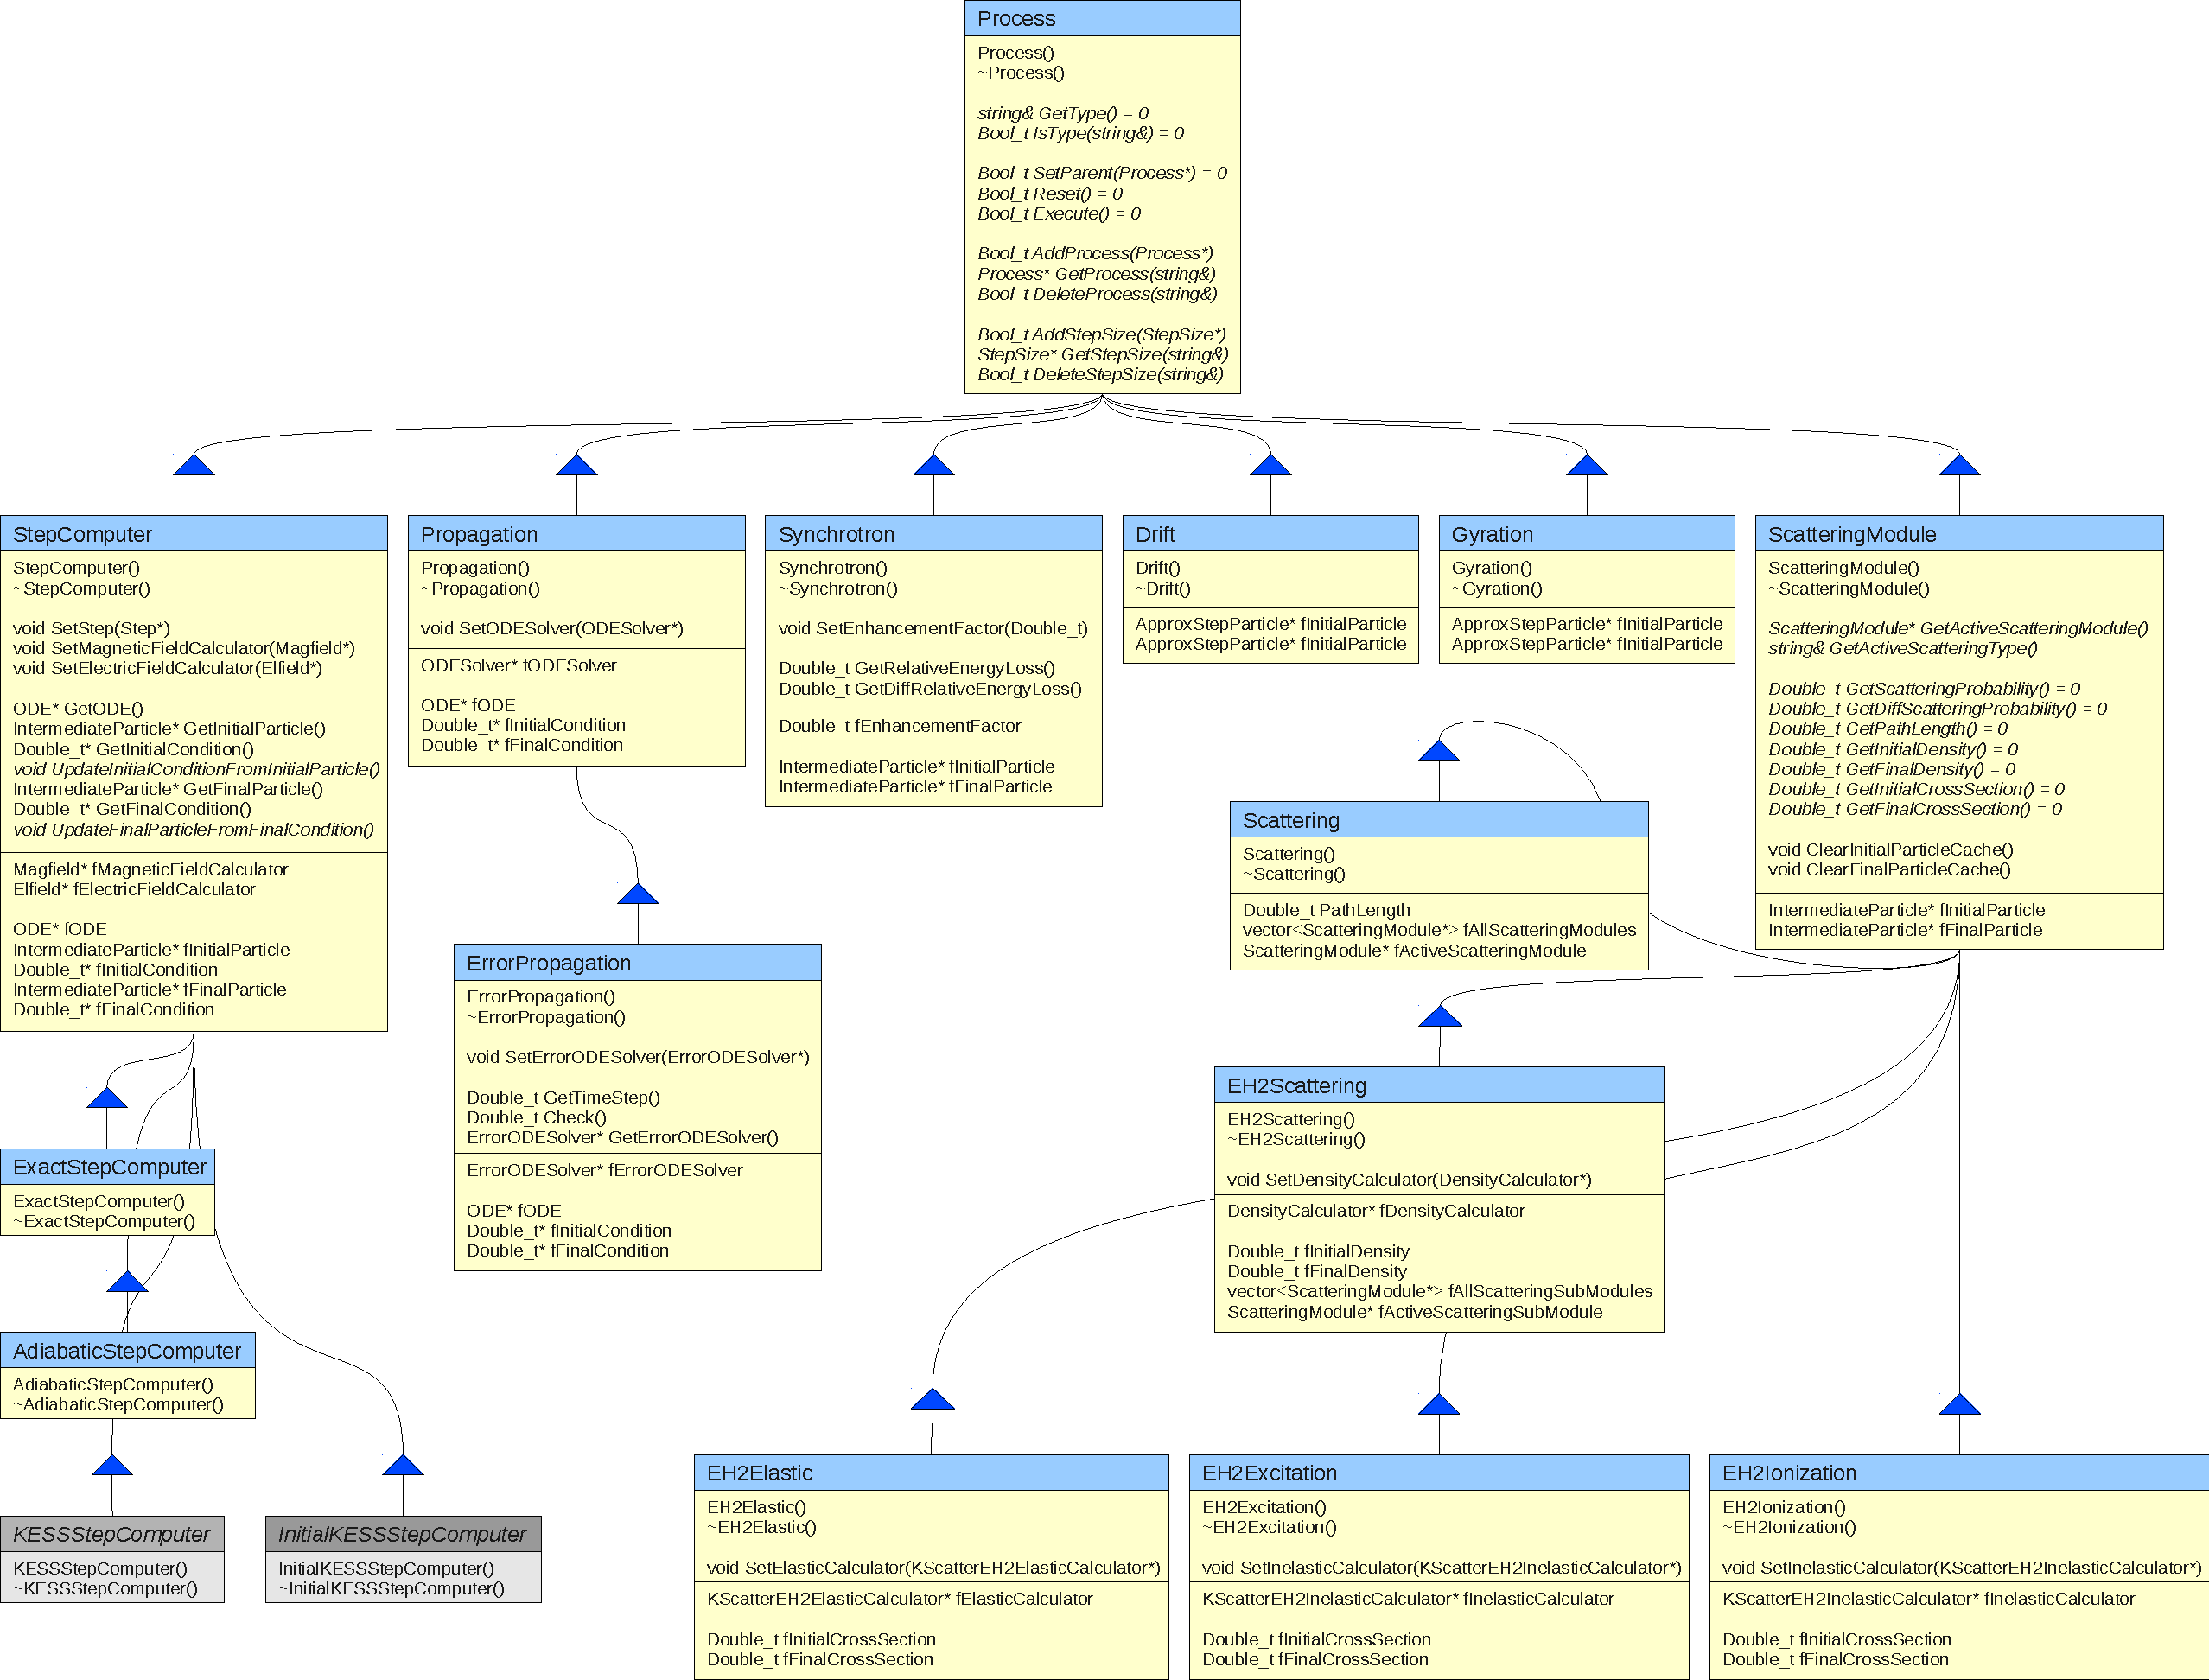
\includegraphics[angle=90,scale=0.58]{./images/KTrackPlots/KTrackProcessInheritance.pdf}
        \caption{Process inheritance diagram for KTrack}
    \end{figure}

\newpage
\thispagestyle{empty}
    \begin{figure}[t]
        \vspace*{-3.5cm}
        \hspace*{-3.2cm}
        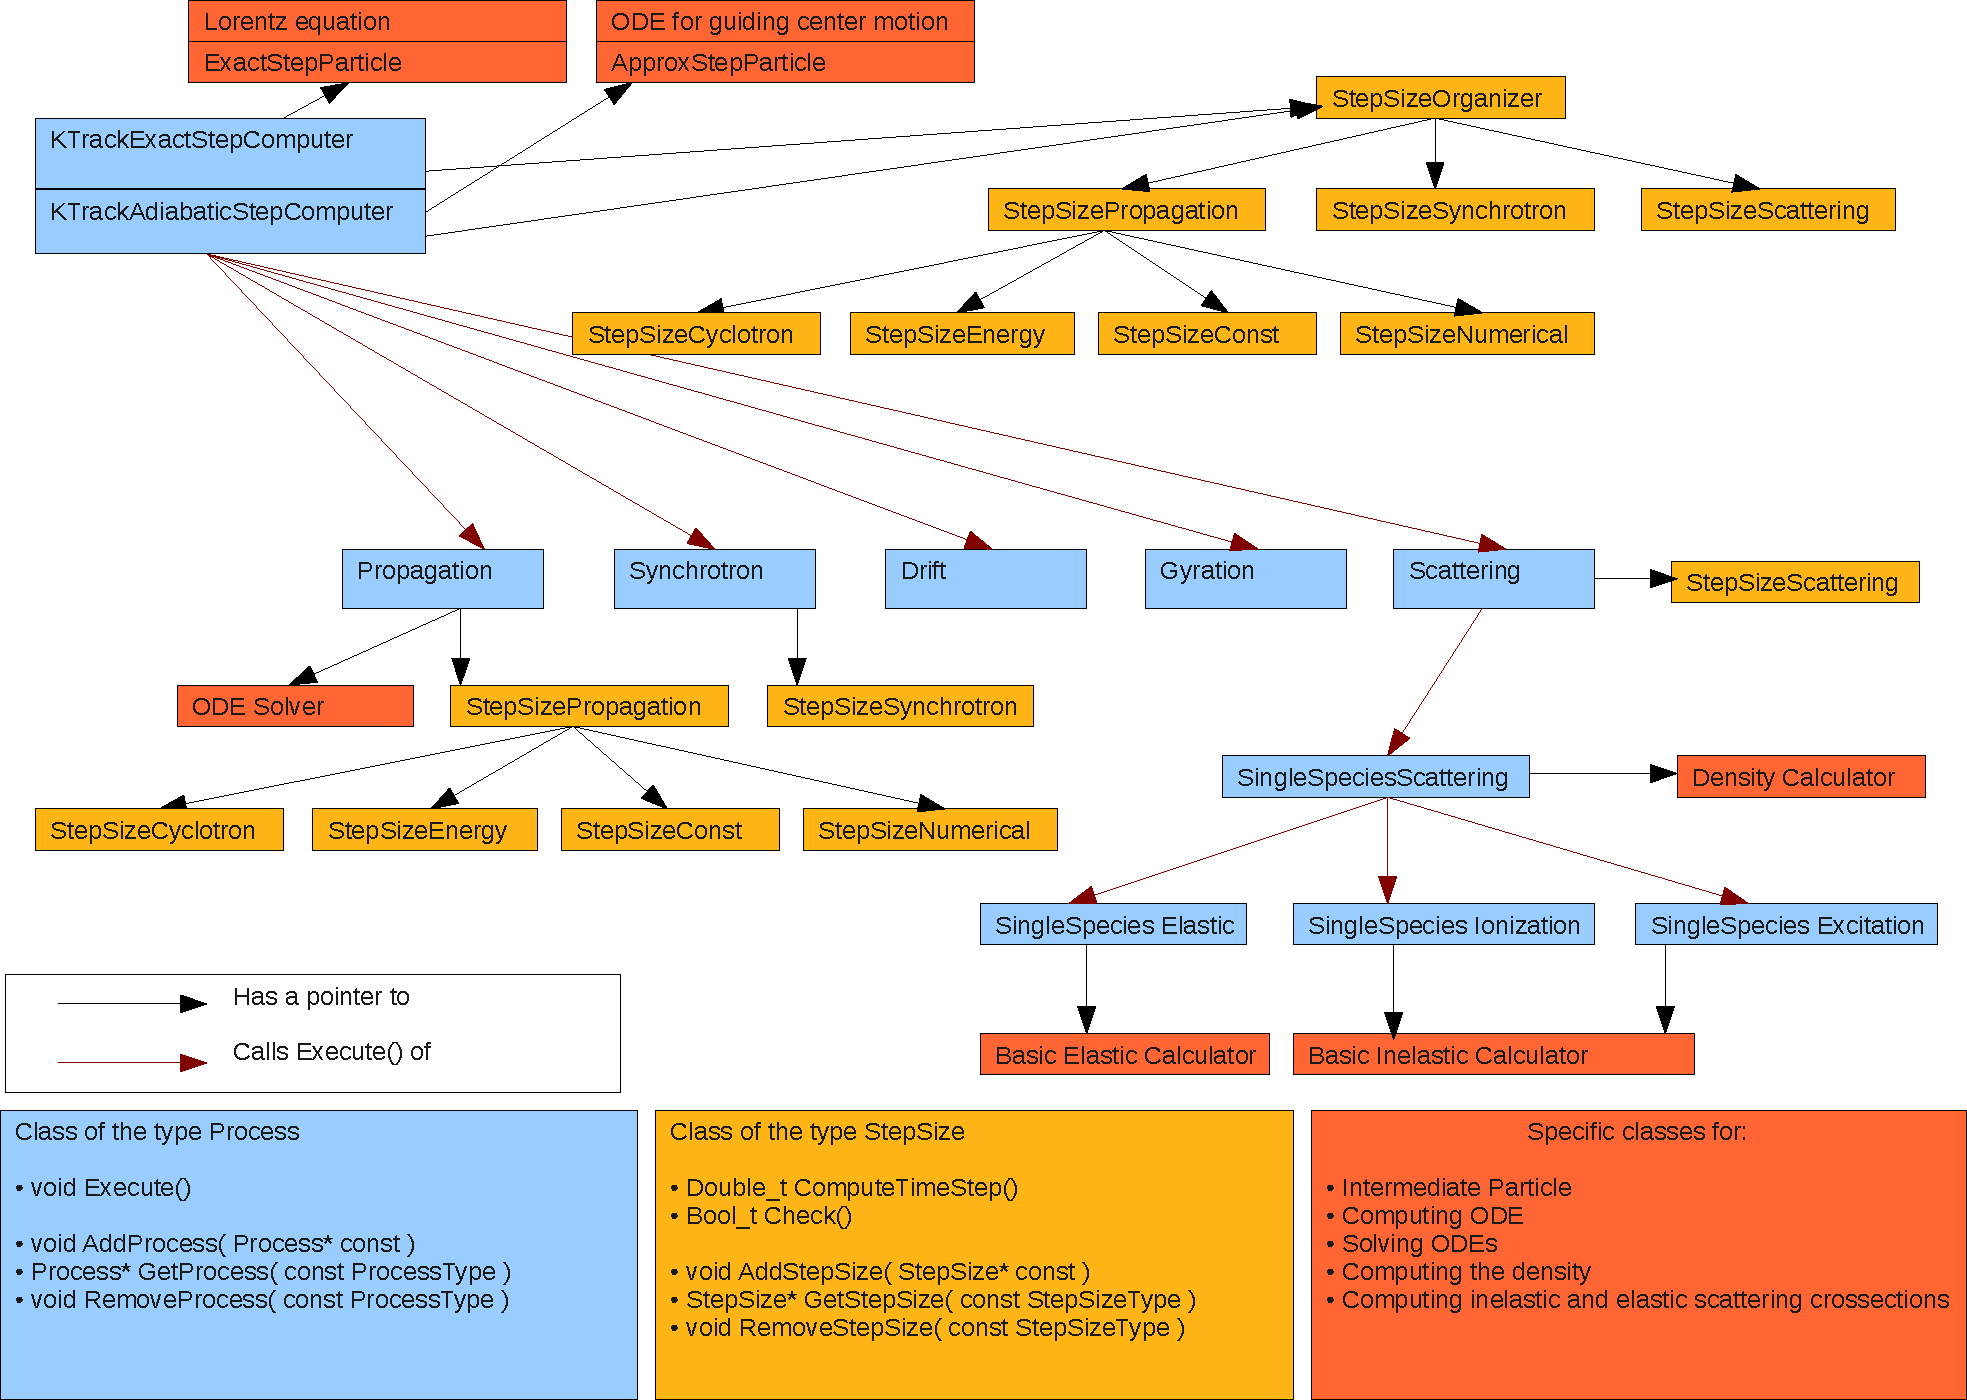
\includegraphics[angle=90,scale=0.75]{./images/KTrackPlots/KTrackDiagramNew.pdf}
        \caption{Collaboration diagram for KTrack}
    \end{figure}


\subsection{Standard test programs}
The purpose of the standard test programs is to give the user and code developer the chance to check whether changes or code developments affected the operability of the program.  

    \subsubsection*{Test against exact track}
    \label{testcompare}
    This test compares different tracking modes against a very accurate exact track. This track is computed using: 
    \begin{itemize}
        \item Exact stepping method
        \item RK8
        \item 48 steps per gyration
    \end{itemize}
    The user can set the conditions for the track that is to be tested:  
    \begin{itemize}
        \item Initial conditions: transmitted or trapped
        \item Stepping method 
        \item ODE solver
        \item Step size control
    \end{itemize}
    When running the test program a trajectory is computed with the chosen method and in addition with the reference settings. At each step of the test trajectory the program determines the position of the particle of the reference track at exactly the time of the test track via interpolation. The absolute value of the difference of the positions is the error.
    
    This test is applicable for short trajectories. For long tracks, e.g. from tracked particles the numerical error of each steps accumulates and will lead to large discripencies between two different tracking methods. Since we do not know the true position of the particle after a long time, another measure of accuracy has to be found. Global variables, like storage time, number of secondary particles, energy loss due to synchrotron, average radius at a given z-position, etc. can be chosen. In section \ref{testtrapped} these tests will be described.
        
    How to use it: Go to directory \textit{Kassiopeia/branches/DanSusanneBranch/bin}. Type \textit{./TestCompareWithExact} this will show you what your options are. Type \textit{./TestCompareWithExact x x x x x x x}, where x is an integer that defines the modes you have chosen. The program writes the deviation of the positions, radius, timestep, etc. between test and reference track into a root file: \textit{Trackxxxxxxx.root}. In addition it automatically creates a plot that shows the deviation over time.
    
    This program was used for testing the operability of the version of KTrack described in this document. In addition the test program was used to test the old version of KTrack. Furthermore, the same analysis was used to cross check old and new KTrack version and singletraj.

    
    \subsubsection*{Test CPT reversal}
    \label{testtime}
     This purpose of this test (\textit{TestCPTReversal}) is to ensure that the KTrack's computational approximations of the underlying
     physical processes do not violate the fundamental symmetries of charge, parity, and time reversal. 
     The user can select the following options to be tested:
    \begin{itemize}
     \item The stepping method: either exact, or using the adiabatic approximation.
     \item The ODE solver
     \item The method of step size control
     \item The electromagnetic field: either uniform constant electric and magnetic fields, or the prespectrometer fields      
    \end{itemize}
    This test program first computes the trajectory of a test particle with the options specified by the user. The
    test particle is an electron, whose initial conditions place it at the origin, with its momentum directed parallel
    to the vector (1,1,1). The electron is propagated for 10$^{5}$ steps and its final position and momentum are recorded.
    Then the test program performs a charge reversal by replacing the electron with a positron, a parity reversal, and a 
    time reversal on the inital conditions and electromagnetic fields. Then the positron is tracked for 10$^{5}$ steps and
    its final position and momentum are compared with that of the previously calculated electron. Since electromagnetism is
    invarient under a simultaneous reversal of charge, parity and time, the final states (position and momentum) of the electron
    and positron should be identical.

    How to use it: From the top level directory go to the \textit{./bin} directory. Type \textit{./TestCPTReversal} to display the available
    options and their corresponding values. Type \textit{./TestCPTReversal x x x x x y} where \textit{x} are the desired option indices
    and \textit{y} is the initial energy of the test particle. The the program will output the final states of the electron and the positron. 
    If their finals states are not identical, or within a very small round off error then some KTrack process has been implemented/changed 
    incorrectly. If further analysis beyond this simple check is desired the trajectory information (x,y,z,t) of the tracked electron
    can be found in a .root file in the same directory with the name \textit{CPTReversalElectronxxxx\_yeV.root}, the track information of 
    the positron is stored in a .root file named \textit{CPTReversalPositronxxxx\_yeV.root}. 
    Note: The synchotron radiation process is not present in this program.      
    
    \subsubsection*{Test of scattering}
    \label{testscatter}
    taken out, since loading pictures caused problems. Will be fixed soon.


    \subsubsection*{Test of synchrotron radiation}
    \label{testtrapped}
    Will be written soon

    
    \subsubsection*{Test of trapped particles}
    \label{testtrapped}
    Will be written soon

\subsection{Tests of KTrack}
    \subsubsection*{Comparison to singletraj}
    
    \textit{Singletraj} is the original tracking program written in C by Ferenc Gl\"uck. A user interface was implemented by Florian Fr\"ankle and Nancy Wandkowsky.
    Four different settings of \textit{singletraj} have been compared to the new KTrack version. 
    \begin{itemize}
        \item Exact stepping mode with fixed time step of $10^{-12} s $.
        \item Exact stepping mode with 32 steps per gyration
        \item Exact stepping mode with energy conservation controlled step size (limits: $10^{-8}, 10^{-12}$)
        \item Adiabatic stepping mode with energy conservation controlled step size (limits: $10^{-8}, 10^{-12}$)
    \end{itemize}
    
    To test the speed of both programs an electron was stored for $10^{-4} s$ in the main spectrometer. The electrons, with the initial conditions :
    \begin{itemize}
        \item $\vec{x}_{\mathrm{start}} = (0,0,0)$,
        \item $E_{\mathrm{kin}_{\mathrm{start}}} = 2000 eV$,
        \item starting angle: $\Phi = 15°$, $\Theta = 0°$
    \end{itemize}
     are magnetically stored between $-9m$ and $+9m$ from the anayzing plane. To get a reliable time measurement the trajectory calculation was repeated ten times and the average run time was computed. Table \ref{speedSingleKTrack} shows the results.
	\begin{center} 
    \begin{table}[t]
        \begin{tabular}{|l||l|l|}
            \hline
             & Singletraj & KTrack \\
            \hline
            \hline
            Exact; Cyclotron & 10.6 s & 5.2 s \\
            \hline
            Exact; Energy & 4.6 s & 2.1 s \\
            \hline
            Adiabatic; Energy & 1.34 s & 0.58 s \\
            \hline
        \end{tabular}
        \caption{This table compares the computation time of singletraj and KTrack. An electron that is trapped for $10^{-4} s$ in the main spectrometer is simulated. See text above.}
        \label{speedSingleKTrack}
    \end{table}
	\end{center}

    
    To test the accuracy, the positions of an electron being transmitted through the main spectrometer are compared. The position is compared at each step and at equal times. The starting conditions of the electrons are:
    \begin{itemize}
        \item $\vec{x}_{\mathrm{start}} = (0,0,-12.5)$,
        \item $E_{\mathrm{kin}_{\mathrm{start}}} = 20000 eV$,
        \item starting angle: $\Phi = 3°$, $\Theta = 0°$ 
    \end{itemize} 

    pictures taken out, since loading caused problems. Will be fixed soon.

\subsection{Technical details}
This chapter will be written in the near future.
    \subsubsection*{Inheritance}
    \label{inheritance}
    \subsubsection*{Const}
    \label{const}
    \subsubsection*{Caching pattern}
    \label{cachingpattern}
    \subsubsection*{Composite pattern}
    \label{compositepattern}    